\graphicspath{{./images/}}
\begin{definition}[Separated, Disconnected, Connected]
    \routineMS.
    \begin{enumerate}[$(i)$]
        \item Two sets $A,B \subseteq X$ are said to be disjoint if $A\cap B = \emptyset$.
        \item Two sets $A,B \subseteq X$ are said to be separated if $\overline{A}\cap B = \emptyset = A \cap \overline{B}$.
        \item A set $E\subseteq X$ is said to be disconnected if it can be written as a union of two nonempty separated sets $A$ and $B$ $(E=A\cup B)$.
        \item A set $E\subseteq X$ is said to be connected if it is not disconnected.
    \end{enumerate}
\end{definition}

\begin{example}
    Consider $\R$ with the standard metric.
    \begin{enumerate}[$*)$]
        \item $A=(1,2)$ and $B=(2,5)$ are serparated.
        \begin{align*}
            &\overline{A}\cap B = [1,2] \cap (2,5) = \emptyset \\
            &A\cap \overline{B} = (1,2) \cap [2,5] = \emptyset \\
            &\implies E=A\cup B \text{ is disconnected.}
        \end{align*}

        \item $C = (1,2]$ and $D-(2,5)$ are disjoint but not separated.
        \begin{align*}
            &C \cap \overline{D} = (1,2] \cap [2,5] = \{2\} \\
            &C \cup D = (1,5) \text{ is indeed connected.}
        \end{align*}
    \end{enumerate}
\end{example}

\begin{theorem}
    \label{thm2.47}
    The following are equivalent:
    \begin{enumerate}[$(i)$]
        \item A nonempty subset of $\R$ is connected $\iff$ it is a singleton or an interval.
        \item Let $E\subseteq \R$. $E$ is connected $\iff$ if $x,y\in E$ and $x < z < y$, then $z\in E$.
    \end{enumerate}
\end{theorem}
\begin{proof}
    HW 6 \qed
\end{proof}
So, in $\R$, connected $\iff$ interval $\iff$ path connected.

\begin{definition}[Perfect Set]
    \routineMS and let $E\subseteq X.$.
    \begin{enumerate}[$(i)$]
        \item $E$ is said to be perfect if $E' = E$.
        \item $E$ is said to be perfeect if $E' \subseteq E$ and $E\subseteq E'$.
        \item $E$ is said to be perfect if $E$ is closed and every point of $E$ is a limit point.
        \item $E$ is said to be perfect if $E$ is closed and $E$ does not have isolated points.
    \end{enumerate}
\end{definition}

\begin{example} \leavevmode \\
    \begin{enumerate}[$*)$]
        \item $E=[0,1] \implies E' = [0,1]$, so $E=E' \implies E$ is perfect.
        \item $E=[0,1]\cup \{2\} \implies 2$ is an isolated point of $E \implies E$ is not perfect.
        \item $E=\{\frac{1}{n} : n\in \N\} \implies E' = {0}$ so $E \not = E',$ so $E$ is not perfect. Is $E'$ perfect?
        $$E' = {0} \implies (E')' = \emptyset, \text{ so $E'$ is not perfect.}$$
    \end{enumerate}
\end{example}

\begin{theorem}
    \label{thm2.43}
    Let $P$ be a nonempty perfect set in $\R^k$. Then $P$ is uncountable. (An exmaple of an immediate consequence: $[0,1]$ is uncountable)
\end{theorem}
\begin{proof}
    In our proof, we will use the following Lemmas:
    \begin{lemma}
        \label{lemma1}
        \routineMS and let $E\subseteq X$ be perfect. If $V$ is any open set in $X$ \st $V\cap E \not = \emptyset$, then $V\cap E$ is an infinite set.
    \end{lemma}
    \begin{proof}
        Let $q\in V\cap E.$ Then
        \begin{equation*}
            \begin{cases*}
                q \in V \implies \exists \delta > 0 \st \nbhd{\delta}{a} \subseteq V \\
                q \in E \implies q \in E'
            \end{cases*}
            \tag{$1$}
        \end{equation*}
        \begin{equation*}
            q \in E' \implies \nbhd{\delta}{q}\cap E \text{ is an infinite set.}
            \tag{$2$}
        \end{equation*}
        $(1),(2) \implies V\cap E$ is infinite.\qed
    \end{proof}

    \begin{lemma}
        \label{lemma2}
        Let $q\in \R^k$. Let $r > 0.$ Then
        $$\overline{\nbhd{r}{q}}=\overline{\{z\in \R^k : \|z-q\|_2 < r\}} = \{z\in \R^k : \|z-q\|_2 \leq r\} = C_r(q).$$
    \end{lemma}
    \begin{proof}
        HW 6 \qed
    \end{proof}

    Notice that
    $$
    \begin{rcases*}
        P' = P \\
        P \not = \emptyset
    \end{rcases*}
    \implies P' \not = \emptyset \implies P \text{ is infinite.}
    $$
    Assume for contradiction $P$ is countable. Let's denote the distinct elements of $P$ by $x_1, x_2, x_3,... :$
    $$P=\{x_1, x_2, x_3,...\}$$
    In what follows, we will construct a sequence of neighborhoods $V_1, V_2, V_3,... \st$
    \begin{enumerate}[$(i)$]
        \item $\forall n \in \N ~~\overline{V} \subseteq V_n$
        \item $\forall n \in \N ~~x_n \not \in \overline{V_{n+1}}$
        \item $\forall n \in \N ~~V_n \cap P \not \in \emptyset$
    \end{enumerate}
    First, let's assume we have constructed these neighborhoods.
    Then for each $n\in\N$, let
    $$K_n = \overline{V_n} \cap P \not = \emptyset$$
    Note that
    \begin{enumerate}[$(I)$]
        \item $\overline{V_{n+1}} \subseteq V_n \subseteq \overline{V_n}$ so $\overline{V_{n+1}}\cap P \subseteq \overline{V_n} \cap P \implies K_{n+1} \subseteq K_n$ for each $n.$
        \item $\begin{rcases*}
            \overline{V} \text{ is a closed and bounded set in $\R^k \implies \overline{V_n}$ is compact.} \\
            P \text{ is perfect $\implies P$ is closed.}
        \end{rcases*} \implies K_n = \overline{V_n}\cap P \text{ is compact.}$
    \end{enumerate}
    \begin{equation*}
        (I),(II) \overset{Thm 2.36}{\implies} \bigcap \limits_{n=1}^\infty K_n \not = \emptyset
        \tag{$*$}
    \end{equation*}
    Recall that $\forall n, K_n \subseteq P,$ so
    $$\bigcap \limits_{n=1}^\infty K_n \subseteq P$$
    However, if $b\in P$ then $b \not \in \bigcap \limits_{n=1}^\infty K_n$; indeed
    $$b\in P \implies b=x_m \text{ for some $m\in \N$}$$
    But $x_m \not \in \overline{V_{m+1}}$ so $x_m \not \in \overline{V_{m+1}\cap P} = K_{m+1}.$ So $x_m \not \in \bigcap \limits_{n=1}^\infty K_n.$ This tells us
    \begin{equation*}
        \bigcap \limits_{n=1}^\infty K_n = \emptyset
        \tag{$**$}
    \end{equation*}
    $$(*),(**) \implies \text{contradiction.}$$

    It remains to show that there exists a seequence of neighborhoods $V_1, V_2, V_3, ...$ satisfying $(i),(ii),(iii)$. We construct these sequences inductively.

    \begin{description}
        \item[Step 1:] Fix $r_1 > 0.$ Let $V_1 = \nbhd{r_1}{x_1}.$ Clearly, $V_1 \cap P \not = \emptyset$.
        \item[Step 2:] Our goal is to construct a neighborhood $V_2 \st$
        \begin{enumerate}[$(i)$]
            \item $\overline{V_2} \subseteq V_1$
            \item $x_1 \not \in V_2$
            \item $V_2 \cap P \not = \emptyset$
        \end{enumerate}
        We can do this just by using the fact that $V_1 \cap P \not = \emptyset.$.
        \begin{align*}
            V_1 \cap P \not = \emptyset \overset{\text{lem\ref{lemma1}}}{\implies} \exists y_1 \in V_1 \cap P \st y_1 \not = x_1 \\
            y_1 \in V_1 \overset{V \text{ is open}}{\implies} \exists \delta_1 > 0 \st \nbhd{\delta_1}{y_1} \subseteq V_1.
        \end{align*}
        Let $r_2 = \frac{1}{2} \min\{d(x_1,y_1), \delta_1\}.$ Let $V_2 = \nbhd{r_2}{y_1}.$ We claim $V_2$ has all the desired properties. Indeed,
        \begin{enumerate}[$(i)$]
            \item $\begin{aligned}[t]
                \overline{V_2} = \overline{\nbhd{r_2}{y_1}} &= \{z \in \R^k : \|z-y_1\|_2 \leq r_2\} \\
                &\subseteq \{z\in \R^k : \|z-y_1\|_2 < \delta_1\} = \nbhd{\delta_1}{y_1} \text{ since $r_2 < \delta_1$}\\
                &\subseteq V_1
            \end{aligned}$
            \item$d(x_1, y_1) > r_2 \implies x_1 \not \in \overline{\nbhd{r_2}{y_1}} = \{z\in \R^k : \|z-y_1\|_2 \leq r_2\}$
            \item $y_1 \in V_2$ and $y_1 \in P \implies V_2 \cap P \not = \emptyset$
        \end{enumerate}

        \item[Step 3:] Repeat the process to find $V_3$:
        \begin{enumerate}[$(i)$]
            \item $\closure{V_3} \subseteq V_2$
            \item $x_2 \not \in \closure{V_3}$
            \item $V_3 \cap P \not = \emptyset$
        \end{enumerate}
        Similarly, for each $k \geq 3,$ we can construct $V_{k+1}$ using only the fact that $V_k \cap P \not = \emptyset.$
    \end{description}
    \qed
\end{proof}

Consider the following construction:
\begin{description}
    \item[\underline{Stage 0:}]\leavevmode \\
    Let $E_0 = [0,1]$.
\end{description}

\begin{figure}[h]
    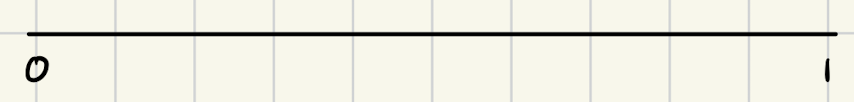
\includegraphics[width=.50\linewidth, center]{/Users/josiahvillarante/GradSchool/Grad-School-Notes/Math230A/Lecture/CH2/images/cantor set 0.png}
\end{figure}

\begin{description}
    \item[\underline{Stage 1:}]\leavevmode \\
    Remove the segment $(\frac{1}{3}, \frac{2}{3})$. That is, remove the middle third of the interval, and define $E_1 = [0, \frac{1}{3}]\cup [\frac{2}{3}, 1]$.
\end{description}

\begin{figure}[h]
    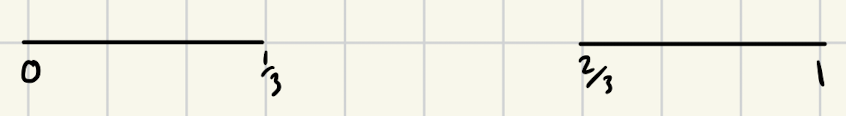
\includegraphics[width=.50\linewidth, center]{/Users/josiahvillarante/GradSchool/Grad-School-Notes/Math230A/Lecture/CH2/images/cantor set 1.png}
\end{figure}

\begin{description}
    \item[\underline{Stage 2:}]\leavevmode \\
    Take each of the intervals $[0, \frac{1}{3}]$ and $[\frac{2}{3}, 1]$ and remove the middle third of each those, and define $$E_2=\left[0, \frac{1}{9}\right]\cup \left[\frac{2}{9}, \frac{3}{9}\right] \cup \left[\frac{6}{9}, \frac{7}{9}\right] \cup \left[\frac{8}{9}, 1\right]$$.
\end{description}

\begin{figure}[h]
    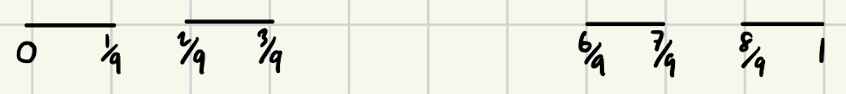
\includegraphics[width=.50\linewidth, center]{/Users/josiahvillarante/GradSchool/Grad-School-Notes/Math230A/Lecture/CH2/images/cantor set 2.png}
\end{figure}

Continuing this process, we will obtain a sequence of compact sets:
$$E_1, E_2, E_3,...$$
\st
\begin{enumerate}
    \item $E_1 \supseteq E_2 \supseteq E_3 \supseteq ...$
    \item For each $n \in \N, ~E_n$ is the union of $2^n$ intervals of length $\frac{1}{3^n}$.
\end{enumerate}

\begin{definition}[The Cantor Set]
    The Cantor set is the set
    $$P= \bigcap \limits_{n=1}^\infty E_n$$
    where each $E_n$ is defined from above.
\end{definition}

\begin{observation}
    Notice that in order to obtain $E_n$, we remove intervals of the form $(\frac{3k+1}{3^n}, \frac{3k+2}{3^n})$.
\end{observation}

\begin{theorem}[Properties of the Cantor set]
Let $P$ denote the Cantor set. Then
\begin{enumerate}[$(i)$]
    \item $P$ is compact
    \item $P$ is nonempty
    \item $P$ contains no segment
    \item $P$ is perfect (and so uncountable)
    \item $P$ has measure zero
\end{enumerate}    
\end{theorem}
\begin{proof}
    \begin{enumerate}[$(i)$]
        \item $P$ is an intersection of compact sets
        \item By Theorem \ref{thm2.36}, the intersection of a sequence of nested, nonempty, compact sets is nonempty
        \item Our goal is to show that $P$ does not contain any set of the form $(\alpha, \beta)$ (where $0 \leq \alpha, ~\beta \leq 1$). Note that, by construction of $P$, the intervals of the form 
        $$I_{k,n} = (\frac{3k+1}{3^n}, \frac{3k+2}{3^n}) ~~n\in\N, ~0\leq k \st 3k+2 < 3^n$$
        have no intersection with $P$.
        However, $(\alpha, \beta)$ contains at least one of $I_{k,n}$'s. Indeed,
        \begin{align*}
            &(\alpha, \beta) \text{ contains $(\frac{3k+1}{3^n}, \frac{3k+2}{3^n})$} \\
            &\iff \alpha < \frac{3k+1}{3^n} \text{ and } \frac{3k+2}{3^n} < \beta \\
            &\iff \frac{3^n \alpha - 1}{3} < k < \frac{3^n \beta - 2}{3}.
        \end{align*}
        So, to ensure $(\alpha, \beta)$ contains aty least one of $I_{k,n}$, it is enough to choose $n\in \N$ \st
        \begin{enumerate}[$(1)$]
            \item $(\frac{3^n\beta - 2}{3}) - (\frac{3^n \alpha -1}{3}) > 1$
            \item $\frac{3^n\beta - 2}{3} > 1$
        \end{enumerate}
        We have
        \begin{enumerate}[$(1)$]
            \item $\iff \frac{3^n(\beta - \alpha) -1}{3} > 4 \iff 3^n (\beta - \alpha) > 4 \iff 3^{-n} < \frac{\beta - \alpha}{4}$
            \item $\iff 3^n \beta - 2 > 3 \iff 3^n \beta > 5 \iff 3^{-n} < \frac{\beta}{5}$
        \end{enumerate}
        So, if we choose $n\in\N \st \frac{1}{3^n} < \min\{\frac{\beta - \alpha}{4}, \frac{\beta}{5}\}$, then we can be sure that $(\alpha, \beta)$ contains $I_{k,n}$ for some positive integer $k$.
        \item $P$ is perfect. We know that $P$ is closed (because it's an intersection of closed sets). So, in order to prove that $P$ is perfect, it is enough to show that every point of $P$ is a limit point of $P$. Let $x\in P$. We want to show $x \in P'$. That is,
        $$\forall \epsilon > 0 ~~\nbhd{\epsilon}{x} \cap (P \backslash \{x\})\not =\emptyset.$$
        We have
        $$x\in P = \bigcap \limits_{n=1}^\infty E_n \implies\forall n \in \N ~x \in E_n \implies \forall n \in \N ~~\exists I_n \subseteq E_n \st x\in I_n.$$
        Choose $n$ large enough \st $|I_n| < \frac{\epsilon}{2}.$ We have
        $$x \in I_n \text{ and $|I_n| < \frac{\epsilon}{2}$} \implies I_n \subseteq (x-\epsilon, x+\epsilon).$$
        At least one of these endpoints of $I_n$ is not $x$, let's call it $y$. Then 
        $$y\in P, ~y\not = x, ~y\in I_n \subseteq(x-\epsilon, x+\epsilon).$$
        So,
        $$y\in (x-\epsilon, x+\epsilon) \cap (P \backslash \{x\}).$$
        Therefore,
        $$(x-\epsilon, x+\epsilon) \cap (P \backslash \{x\}) \not = \emptyset.$$
    \end{enumerate}
    \qed
\end{proof}